\documentclass[a4paper,10pt]{book}

\usepackage[usenames]{color}
\usepackage{bm}
\usepackage{amsmath}
\usepackage{xspace}
\usepackage{a4wide}
\usepackage{wrapfig}
\usepackage[numbers,comma,sort&compress]{natbib}
\usepackage{graphicx}
\usepackage{xstring}
\usepackage{listings,courier}
%\usepackage{draftcopy}
\usepackage{longtable}
\usepackage{paralist}
%\usepackage{fancyvrb}
\usepackage{listings}
\usepackage{array}
\usepackage[table]{xcolor}
\usepackage{units}
\usepackage[toc,page]{appendix}

\definecolor{webgreen}{rgb}{0,.5,0}
\definecolor{webbrown}{rgb}{.6,0,0}
\definecolor{invisiblegray}{rgb}{.97,0.97,0.97}

\usepackage
[dvips, %dvipdf, %or dvips or pdftex 
pagebackref, %or backref
colorlinks=true,
linkcolor=webgreen, %defined below
filecolor=webbrown, %defined below
citecolor=webgreen, %defined below
pdftitle={VOTCA-CT manual},
pdfauthor={},
pdfsubject={VOTCA-CTP},
pdfkeywords={charge transport organic semiconductors},
bookmarksopen=false,
pdfpagemode=UseNone]{hyperref}

%\pdfcompresslevel=9

\usepackage[T1]{fontenc}
%\usepackage{times}
\usepackage{type1cm}

\def\bibsection{%
    \chapter*{Bibliography}%
    \addcontentsline{toc}{chapter}{Bibliography}
}

\begin{document}


\lstset{
  language=XML,
  frame=lines,
  backgroundcolor=\color{invisiblegray},
  basicstyle=\ttfamily\footnotesize,
  identifierstyle=\color{red},
  keywordstyle=\color{blue},
  commentstyle=\color{gray}\rmfamily\itshape,
  mathescape=true,
  morekeywords={estatic_params,estatic_method,epsilon_dielectric,s_eps}
}

\input{hgid}

\newcommand{\equ}[1]{eq.~\eqref{equ:#1}}
\newcommand{\Equ}[1]{Eq.~\eqref{equ:#1}}
\newcommand{\fig}[1]{figure~\ref{fig:#1}}
\newcommand{\Fig}[1]{Figure~\ref{fig:#1}}
\newcommand{\sect}[1]{chapter~\ref{sec:#1}}
\newcommand{\Sect}[1]{Chapter~\ref{sec:#1}}
\newcommand{\slink}[2]{\hyperref[#1]{#2}}
\newcommand\votcalogo{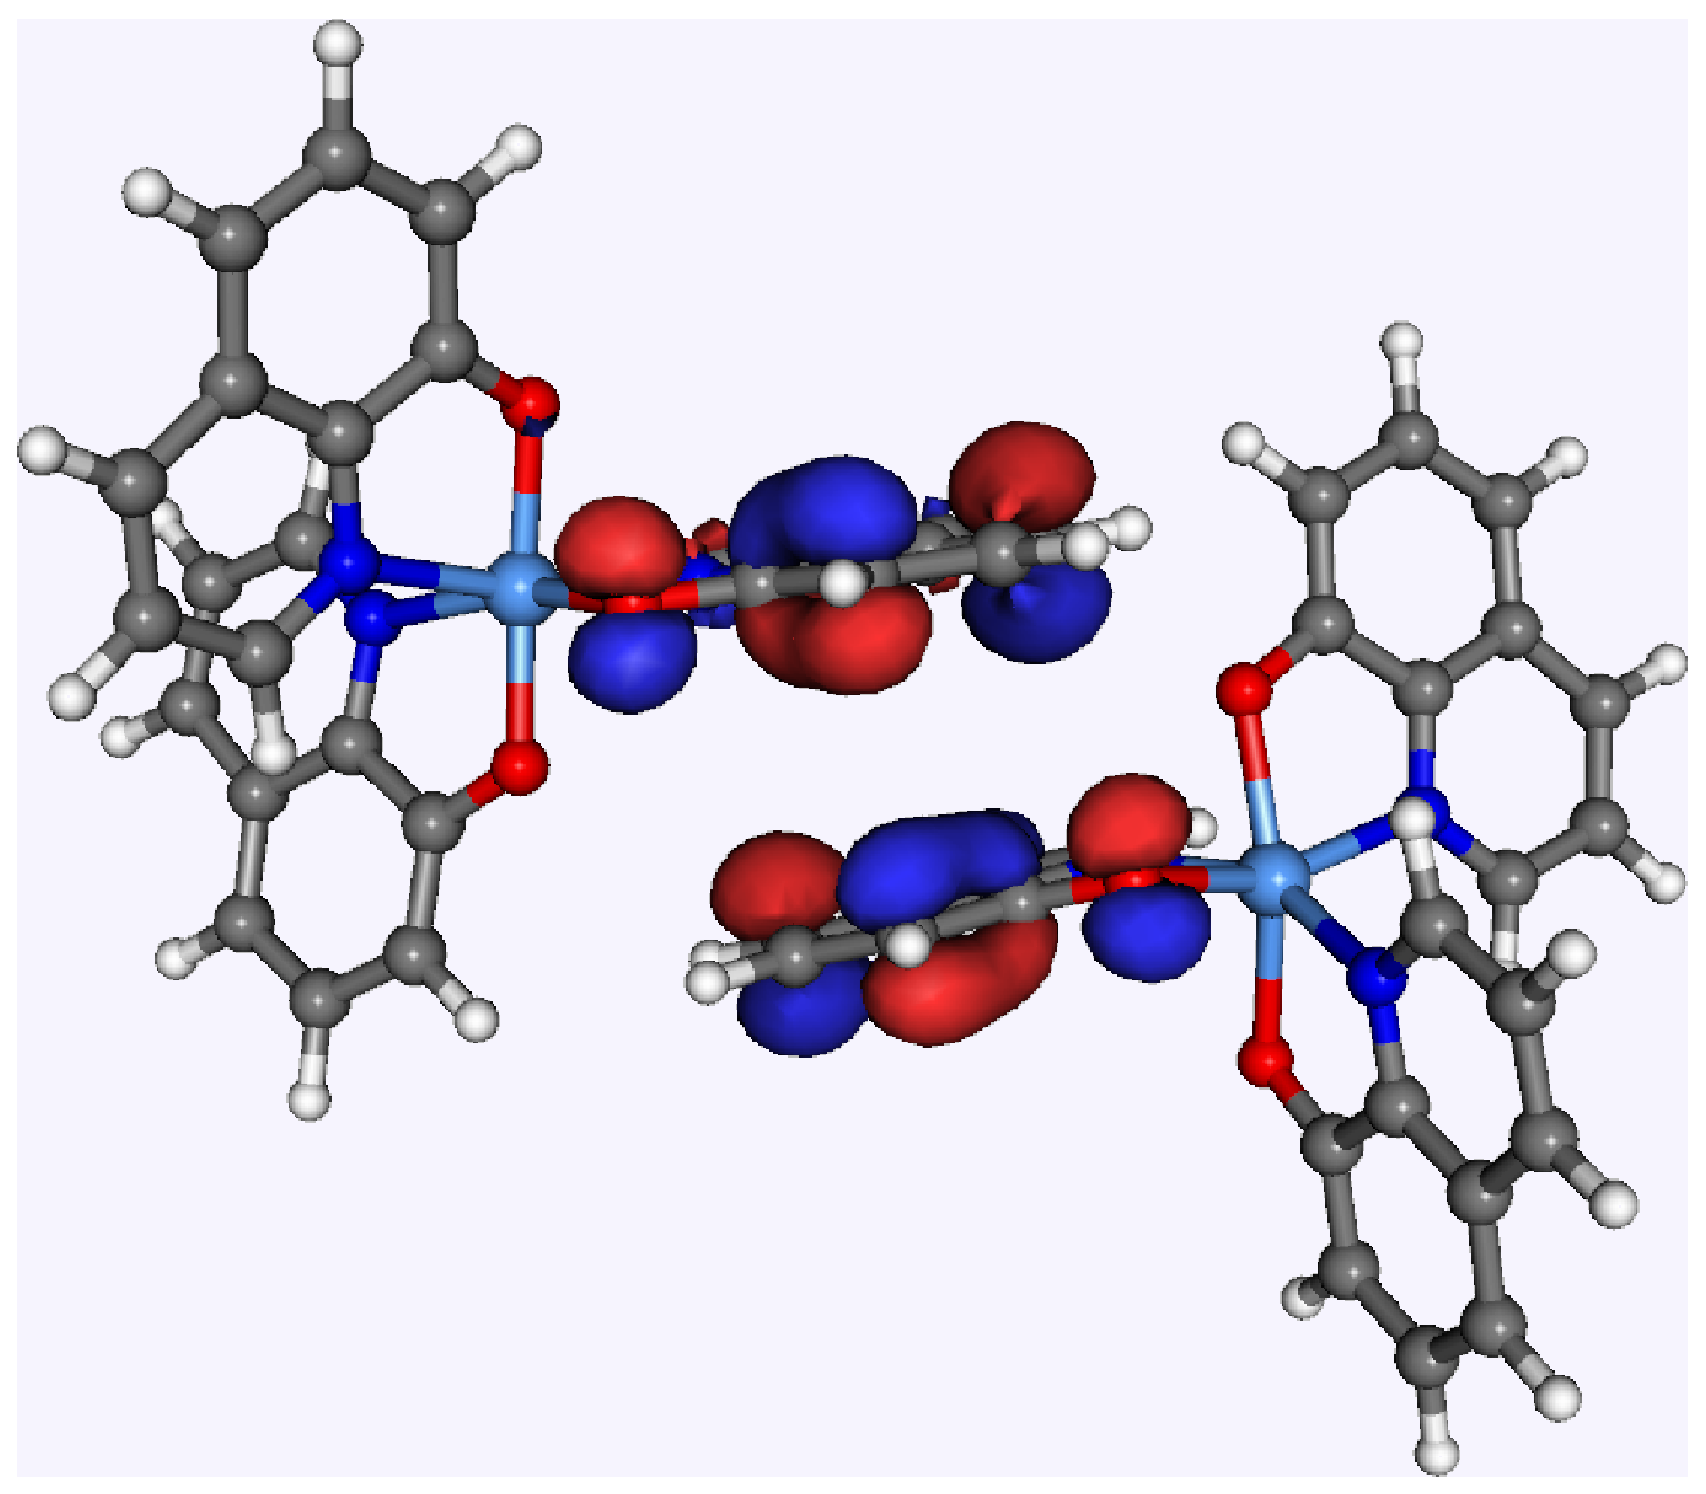
\includegraphics[width=17pt]{fig/logo_trans}}
\newcommand\votcacommand[2]
{
\begin{bclogo}[couleur=mygray, arrondi =0 , logo=\votcalogo, barre=line,noborder=true]{\small #1}
\itshape {\small #2}
\end{bclogo}
}

\newcommand{\xml}{XML\xspace}
\newcommand{\gromacs}{\texttt{GROMACS}\xspace}
\newcommand{\gaussian}{\texttt{Gaussian}\xspace}
\newcommand{\turbomole}{\texttt{Turbomole}\xspace}
\newcommand{\nwchem}{\texttt{NWChem}\xspace}
\newcommand{\tinker}{\texttt{TINKER}\xspace}
\newcommand{\dipro}{\texttt{DIPRO}\xspace}

\newcommand{\Alq}{$\mathrm{Alq}_3$\xspace}
\newcommand{\dcvt}{DCV2T\xspace}

\newcommand{\xyz}{\texttt{geometry.xyz}\xspace}
\newcommand{\orb}{\texttt{zindo.orb}\xspace}
\newcommand{\votcactp}{{\MakeUppercase{votca-ctp}}\xspace}

\newcommand{\calculator}{\hyperref[sec:calculators]{calculator}\xspace}
\newcommand{\tool}{\hyperref[sec:calculators]{tool}\xspace}

\newcommand{\xmloptions}{\texttt{options.xml}\xspace}
\newcommand{\xmlcsg}{\hyperref[sec:xmlmap]{\texttt{map.xml}}\xspace}
\newcommand{\xmlsegments}{\hyperref[sec:xmlsegments]{\texttt{segments.xml}}\xspace}
\newcommand{\sqlstate}{\hyperref[sec:statefile]{\texttt{state.db}}\xspace}
\newcommand{\topology}{\texttt{topol.tpr}\xspace}
\newcommand{\trajectory}{\texttt{traj.xtc}\xspace}

\newcommand{\opt}{\texttt{{ -}o}\xspace}
\newcommand{\seg}{\texttt{{ -}s}\xspace}
\newcommand{\sql}{\texttt{{ -}f}\xspace}
\newcommand{\exe}{\texttt{{ -}e}\xspace}
\newcommand{\tpl}{\texttt{{ -}t}\xspace}
\newcommand{\csg}{\texttt{{ -}m}\xspace}
\newcommand{\trj}{\texttt{{ -}c}\xspace}
\newcommand{\job}{\texttt{{ -}j}\xspace}
\newcommand{\run}{\texttt{{run}}\xspace}
\newcommand{\wrt}{\texttt{{write}}\xspace}
\newcommand{\rd}{\texttt{{read}}\xspace}


\newcommand{\refcalc}{\hyperref[ref:calculators]{calculators}\xspace}

\newcommand{\overlap}{\hyperref[prog:moo_overlap]{\texttt{moo\_overlap}}\xspace}
\newcommand{\ctprun}{\hyperref[prog:ctp_run]{\texttt{ctp\_run}}\xspace}
\newcommand{\ctpmap}{\hyperref[prog:ctp_map]{\texttt{ctp\_map}}\xspace}
\newcommand{\ctpdipro}{\hyperref[prog:ctp_dipro]{\texttt{ctp\_dipro}}\xspace}
\newcommand{\ctpparallel}{\hyperref[prog:ctp_parallel]{\texttt{ctp\_parallel}}\xspace}
\newcommand{\ctpdump}{\hyperref[prog:ctp_dump]{\texttt{ctp\_dump}}\xspace}
\newcommand{\ctpupdate}{\hyperref[prog:ctp_update]{\texttt{ctp\_update}}\xspace}
\newcommand{\ctptools}{\hyperref[prog:ctp_tools]{\texttt{ctp\_tools}}\xspace}
\newcommand{\kmcrun}{\hyperref[prog:kmc_run]{\texttt{kmc\_run}}\xspace}

\newcommand{\sqlite}{\texttt{sqlite3}\xspace}
\newcommand{\sqlconjsegproperties}{\texttt{conjseg\_properties}\xspace}
\newcommand{\sqlconjsegs}{\texttt{conjsegs}\xspace}
\newcommand{\sqlmolecules}{\texttt{molecules}\xspace}
\newcommand{\sqlpairintegrals}{\texttt{pairintegrals}\xspace}
\newcommand{\sqlpairproperties}{\texttt{pairproperties}\xspace}
\newcommand{\sqlpairs}{\texttt{pairs}\xspace}
\newcommand{\sqlrigidfragproperties}{\texttt{rigidfrag\_properties}\xspace}
\newcommand{\sqlrigidfrags}{\texttt{rigidfrags}\xspace}
\newcommand{\sqlframes}{\texttt{frames}\xspace}


\newcommand{\suggestion}[1]{{\color{red}SUGGESTION: #1}}

\newcommand{\segmentref}[1]{segments.#1}
\newcommand{\segmentopt}[1]{\hyperlink{\segmentref{#1}}{\StrSubstitute{#1}{_}{\_}}\xspace}
\newcommand{\calcref}[1]{#1}
\newcommand{\calcopt}[1]{\hyperlink{\calcref{#1}}{\StrSubstitute{#1}{_}{\_}}\xspace}

\newcommand{\calc}[1]{\hyperref[calc:#1]{\texttt{#1}}\xspace}
\newcommand{\toolref}[1]{\hyperref[tool:#1]{\texttt{#1}}\xspace}

\def\bibsection{%
    \chapter*{Bibliography}%
    \addcontentsline{toc}{chapter}{Bibliography}
}

\renewcommand*{\showkeyslabelformat}[1]{{\normalfont\tiny\sffamily#1}}
\definecolor{refkey}{rgb}{1,0,0}
\definecolor{labelkey}{rgb}{1,0,0}

% Calculus and Linear Algbra Notation
% formulas
\newcommand{\vctr}[1]{\mathbf{ \bar{#1} }}
\newcommand{\oper}[1]{\hat{ #1 }}
\newcommand{\matr}[1]{\mathbf{ #1 }}

%% FULL COMMANDS LISTING
\newcommand{\cmdmap}{\ctpmap \tpl \topology \trj \trajectory \seg \xmlcsg  \sql \sqlstate}
\newcommand{\cmdnbl}{\ctprun \opt \xmloptions  \sql  \sqlstate \exe  \calc{neighborlist}}
\newcommand{\cmdemlt}{\ctprun \opt \xmloptions  \sql  \sqlstate \exe  \calc{emultipole}}
\newcommand{\cmdeint}{\ctprun \opt \xmloptions  \sql  \sqlstate \exe  \calc{einternal}}
\newcommand{\cmdedft}{\ctpparallel \opt \xmloptions \sql \sqlstate \exe \calc{edft}}
\newcommand{\cmdidft}{\ctpparallel \opt \xmloptions \sql \sqlstate \exe \calc{idft}}
\newcommand{\cmdizindo}{\ctprun \opt \xmloptions  \sql  \sqlstate \exe  \calc{izindo}}
\newcommand{\cmdouter}{\ctprun \opt \xmloptions  \sql  \sqlstate \exe  \calc{outersphere}}
\newcommand{\cmdrates}{\ctprun \opt \xmloptions  \sql  \sqlstate \exe  \calc{rates}}
\newcommand{\cmdkmc}{ \kmcrun \opt \xmloptions  \sql  \sqlstate \exe  \calc{kmcmultiple}}
\newcommand{\cmdkmcsin}{ \kmcrun \opt \xmloptions  \sql  \sqlstate \exe  \calc{kmcsingle}}
\newcommand{\cmdeana}{\ctprun \opt \xmloptions  \sql  \sqlstate \exe  \calc{eanalyze}}
\newcommand{\cmdmolpol}{\ctptools \opt \xmloptions \exe \toolref{molpol}}
\newcommand{\cmdlogmps}{\ctptools \opt \xmloptions \exe \toolref{log2mps}}
\newcommand{\cmdxqmult}{\ctpparallel \opt \xmloptions \sql \sqlstate \exe \calc{xqmultipole}}



\frontmatter
\begin{titlepage}

%\center{\fontsize{4cm}{5cm}\selectfont VOTCA-CT}
%\center{\fontsize{1.5cm}{3cm}\selectfont USER MANUAL}

\center{\huge \sc Charge Transport Simulations}
\vspace*{1cm}
\center{\Large \sc User Manual}

\vspace*{3cm}
\center{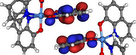
\includegraphics[width=0.6\columnwidth]{fig/logo}}
\vspace*{1cm}

\vfill
{\small% 
If you are using this package please site \\
\vspace*{0.1cm}
V. R\"uhle, A. Lukyanov, F. May, M. Schrader, T. Vehoff, J. Kirkpatrick, B. Baumeier, D. Andrienko \\
``Microscopic simulations of charge transport in disordered organic semiconductors'' \\
\htmladdnormallink{\color{black} {\itshape J. Chem. Theor. Comp.} 2011}
{http://dx.doi.org/} 
%\\
%\vspace*{0.1cm}
%and \\
%\vspace*{0.1cm}
%V. R\"uhle, C. Junghans, A. Lukyanov, K. Kremer, D. Andrienko \\
%``Versatile Object-oriented Toolkit for Coarse-graining Applications'' \\
%\htmladdnormallink{ \color{black} {\itshape J. Chem. Theor. Comp.} 5, 3211, 2009}
%{http://dx.doi.org/10.1021/ct900369w}
}

\vspace*{1.4cm}
\center{\large{\today}}
%\vspace*{-0.3cm}
%\center{\footnotesize{compiled from: \hgid}}
%\center{\footnotesize{Programs version: \refhgid}}

%\vspace*{1cm}
%\center{
%\large{\copyright \hspace*{0.1cm} VOTCA development team}
%}
%\vspace*{0.5cm}



\htmladdnormallink{\color{black}\large{www.votca.org}}{http://www.votca.org}
\end{titlepage}

\thispagestyle{empty}
\cleardoublepage

\tableofcontents
%\cleardoublepage
\mainmatter
\chapter{Introduction}
\label{sec:introduction}

Charge carrier dynamics in an organic semiconductor can often be described in terms of charge hopping between localized states. The hopping rates depend on \slink{transfer_integrals}{electronic coupling elements}, \slink{reorganization}{reorganization energies}, and \slink{site_energies}{driving forces}, which vary as a function of position and orientation of the molecules.  The exact evaluation of these contributions in a molecular assembly is computationally prohibitive. Various, often semi-empirical, approximations are employed instead. The purpose of the \votcactp package~\cite{ruehle_microscopic_2011} is to simplify the workflow for charge transport simulations, provide a uniform error-control for the methods, flexible platform for their development, and eventually allow in silico prescreening of organic semiconductors for specific applications. 

The toolkit is implemented using modular concepts introduced earlier in the Versatile Object-oriented Toolkit for Coarse-graining Applications (VOTCA)~\cite{ruehle_versatile_2009}. The VOTCA structures are adapted to reading atomistic trajectories, mapping them onto \slink{segments}{conjugated segments and rigid fragments}, and substituting (if needed) rigid fragments with the optimized copies. 

The \slink{izindo}{molecular orbital overlap} module calculates electronic coupling elements between  conjugated segments from the corresponding molecular orbitals. It relies on the semi-empirical INDO Hamiltonian and molecular orbitals in the format provided by the \gaussian package. An alternative,  \slink{dft}{density-functional} based approach, has interfaces to the \gaussian and \turbomole packages. An interface to the \tinker package is provided for calculations of electrostatic and polarization contributions to \slink{site_energies}{energetic disorder}. 

The  \slink{kmc}{kinetic Monte Carlo} module reads in the \slink{neighborlist}{neighbor list}, \slink{morphology}{site coordinates}, and \slink{rates}{hopping rates} and performs charge dynamics simulations using either periodic boundary conditions or charge sources and sinks. 

The toolkit is written as a combination of modular C++ code and scripts. The data transfer between programs is implemented via a \slink{statefile}{state file} (sql database), which is also used to restart simulations. Analysis functions and most of the calculation routines are encapsulated by using the observer pattern~\cite{gamma_design_1995} which allows the implementation of new functions as individual modules.
\chapter{Theoretical background}
\label{sec:theory}

\section{Workflow}
\label{sec:wokflow}

A typical workflow of charge transport simulations is depicted in \fig{workflow}. The first step is the simulation of an \slink{morphology}{atomistic morphology}, which is then partitioned on \slink{segments}{hopping sites}. The coordinates of the hopping sites are used to construct a list of pairs of molecules, or \slink{neighborlist}{neighbor list}. 

\begin{figure}[h]
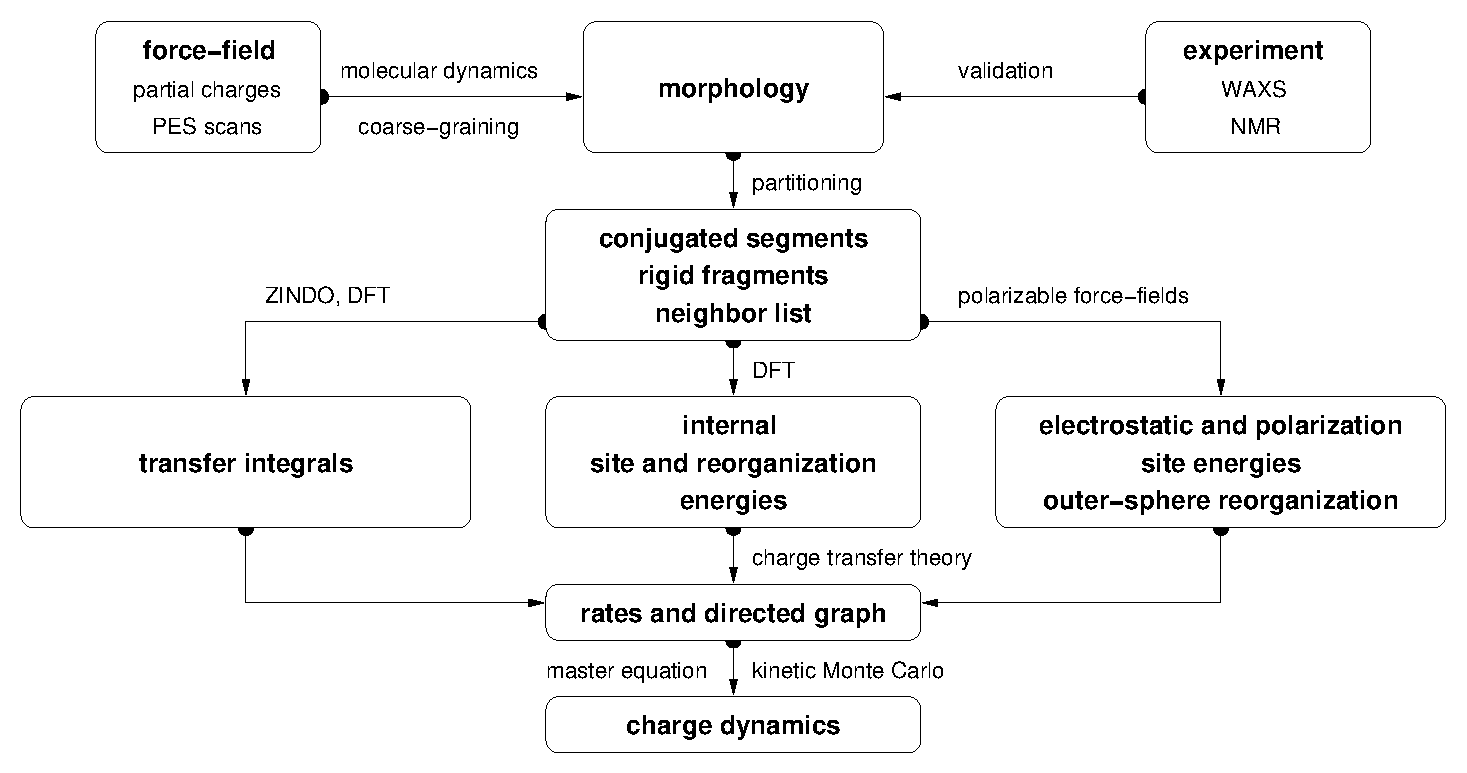
\includegraphics[width=\textwidth]{fig/workflow/workflow}
 \caption{%
   Workflow for microscopic simulations of charge transport.  %
   \label{fig:workflow}}
\end{figure}

For each pair an \slink{transfer_integrals}{electronic coupling element}, a \slink{reorganization}{reorganization energy}, a \slink{site_energies}{driving force}, and eventually the \slink{rates}{hopping rate} are evaluated. The neighbor list and hopping rates define a directed graph. The corresponding master equation is solved using the \slink{kmc}{kinetic Monte Carlo} method, which allows to explicitly monitor the charge dynamics in the system as well as to calculate time or ensemble averages of occupation probabilities, charge fluxes, correlation functions, and field-dependent mobilities.

\section{Material morphology}
\label{sec:morphology}

There is no generic recipe on how to predict a large-scale atomistically-resolved morphology of an organic semiconductor. The required methods are system-specific: for ultra-pure crystals, for example, density-functional methods can be used provided the crystal structure is known from experiment. For partially disordered organic semiconductors, however, system sizes much larger than a unit cell  are required. Classical molecular dynamics or Monte Carlo techniques are then the methods of choice. 

In molecular dynamics, atoms are represented by point masses which interact via empirical potentials prescribed by a force-field. Force-fields are parametrized for a limited set of compounds and their refinement is often required for new molecules. In particular, special attention shall be paid to torsion potentials between successive repeat units of conjugated polymers or between functional groups and the $\pi$-conjugated system. First-principles methods can be used to characterize the missing terms of the potential energy function. 

Self-assembling materials, such as soluble oligomers, discotic liquid crystals, block copolymers, partially crystalline polymers, etc., are the most complicated to study. The morphology of such systems often has several characteristic length scales and can be kinetically arrested in a thermodynamically non-equilibrium state. For such systems, the time- and length-scales of atomistic simulations might be insufficient to equilibrate or sample desired morphologies. In this case, systematic coarse-graining can be used to enhance sampling~\cite{ruehle_versatile_2009}. Note that the coarse-grained representation must reflect the structure of the atomistic system and allow for back-mapping to the atomistic resolution.

Here we assume that the morphology is already known, that is we know how the topology and the coordinates of all atoms in the systems at a given time. \votcactp can read standard \gromacs topology files. Custom definitions of \slink{atomistic}{atomistic topology} via \xml files are also possible. Since the description of the atomistic topology is the first step in the charge transport simulations, it is important to follow simple conventions on how the system is partitioned on molecules, residues, and how atoms are named in the topology. Required input files are described in section \slink{atomistic}{atomistic topology}. 

\section{Conjugated segments and rigid fragments}
\label{sec:segments}

\begin{figure}
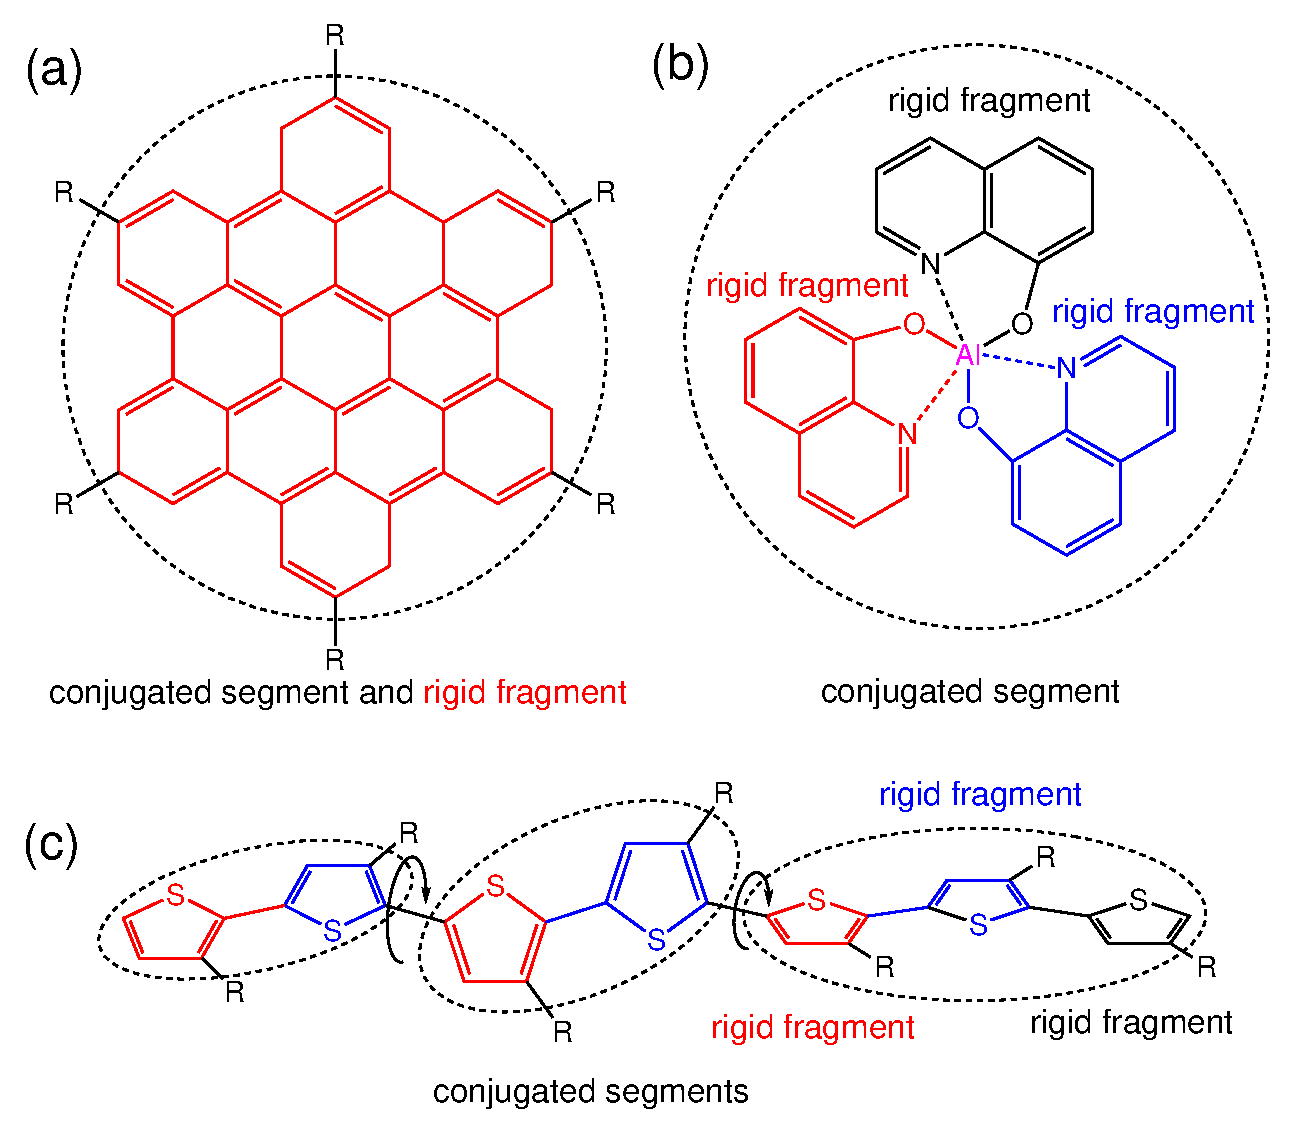
\includegraphics[width=\linewidth]{fig/conjugated_segment/fragment_segment}
\caption{The concept of conjugated segments and rigid fragments. Dashed lines indicate conjugated segments while colors denote rigid fragments. (a) Hexabenzocoronene: the $\pi$-conjugated system is both a rigid fragment and a conjugated segment. (b) \Alq: the Al atom and each ligand are rigid fragments while the whole molecule is a conjugated segment. (c) Polythiophene: each repeat unit is a rigid fragment. A conjugated segment consists of one or more rigid fragments. One molecule can have several conjugated segments.}
\label{fig:segment}
\end{figure}

With the morphology at hand, the next step is partitioning the system on hopping sites\index{hopping site}, or conjugated segments\index{conjugated segment}, and calculating charge transfer rates between them. Physically intuitive arguments can be used for the partitioning,  which reflects the localization of the wave function of a charge. For most organic semiconductors, the molecular architecture includes relatively rigid, planar $\pi$-conjugated systems, which we will refer to as rigid fragments. A conjugated segment can contain one or more of such rigid fragments, which are linked by bonded degrees of freedom. The dynamics of these degrees of freedom evolves on timescales much slower than the frequency of the internal promoting mode. In some cases, e.g. glasses, it can be `frozen' due to non-bonded interactions with the surrounding molecules.

To illustrate the concept of conjugated segments and rigid fragments, three representative molecular architectures are shown in \fig{segment}. The first one is a typical discotic liquid crystal, hexabenzocoronene. It consists of a conjugated core to which side chains are attached to aid self-assembly and solution processing. In this case the orbitals localized on side chains do not participate in charge transport and the conjugated $\pi$-system is both, a rigid fragment and a conjugated segment. 
%
In \Alq, a metal-coordinated compound, a charge carrier is delocalized over all three ligands. Hence, the whole molecule is one conjugated segment. Individual ligands are relatively rigid, while energies of the order of $k_\text{B}T$ are sufficient to reorient them with respect to each other. Thus the Al atom and the three ligands are rigid fragments.
%
In the case of a conjugated polymer, one molecule can consist of several conjugated segments, while each backbone repeat unit is a rigid fragment. Since the conjugation along the backbone can be broken due to large out-of-plane twists between two repeat units, an empirical criterion, based on the dihedral angle, can be used to partition the backbone on conjugated segments~\cite{ruhle_multiscale_2010}. However, such intuitive partitioning is, to some extent, arbitrary and shall be validated by other methods~\cite{vukmirovic_charge_2008,vukmirovic_charge_2009,mcmahon_ad_2009}. 

After partitioning, an additional step is often required to remove bond length fluctuations introduced by molecular dynamics simulations, since they are already integrated out in the derivation of the rate expression. This is achieved by substituting respective molecular fragments with  rigid, planar $\pi$-systems\index{rigid fragment} optimized using first-principles methods. Centers of mass and gyration tensors are used to align rigid fragments, though a custom definition of local axes is also possible. Such a procedure also minimizes discrepancies between the force-field and first-principles-based ground state geometries of conjugated segments, which might be important for calculations of electronic couplings, reorganization energies, and intramolecular driving forces. 

To partition the system on hopping sites and substitute rigid fragments with the corresponding ground-state geometries \ctpmap program is used:
\votcacommand{Mapping the \gromacs trajectory}{\cmdmap}
It reads in the \gromacs topology (\topology) and trajectory (\trajectory) files, definitions of conjugated segments and rigid fragments (\xmlcsg) and outputs coordinates of conjugated segments (hopping sites) and rigid fragments (as provided in the MD trajectory and after rigidification) to the  state file (\sqlstate). In order to do this, a mapping file \xmlcsg has to be provided, which specifies the corresponding atoms in the different representations. After this step, all information (frame number, dimensions of the simulation box, etc) are stored in the \slink{statefile}{state file} and only this file is used for further calculations.

\attention{\votcactp requires a wrapped trajectory for mapping the segments and fragments, so all molecules should be whole in the frame.}   

In order to visually check the mapping one can use either the \calc{tdump} \calculator or the programm \ctpdump with the calculator \calc{trajectory2pdb}.

\label{sec:ctp_dump}
\votcacommand{Writing a mapped trajectroy with \ctpdump}{\small \ctpdump \sql \sqlstate \exe \calc{trajectory2pdb} }

It reads in the state file created by \ctpmap and outputs two trajectory files corresponding to the original and rigidified atom coordinates. To check the mapping, it is useful to superimpose the three outputs (original atomistic, atomistic stored in the state file, and rigidified according to ground state geometries), e.g., with {\tt VMD}.

\label{sec:tdump}
\votcacommand{Writing a mapped trajectroy with \calc{tdump} }{\small \ctprun \sql \sqlstate \opt \xmloptions \exe \calc{tdump} }

It also reads in the state file but appends the coordinates to a pdb. file. So make sure to delete old QM.pdb and MD.pdb if you want to create a new imagef



\section{Neighbor list}
\label{sec:neighborlist}

A list of neigboring conjugated segments, or neighbor list\index{neighbor list}, contains all pairs of conjugated segments for which \slink{sec:transfer_integrals}{coupling elements}, \slink{sec:reorganization}{reorganization energies}, \slink{sec:site_energies}{site energy differences}, and \slink{sec:rates}{rates} are evaluated.

Two segments are added to this list if the distance between centers of mass of any of their rigid fragments is below a certain cutoff. This allows neighbors to be selected on a criterion of minimum distance of approach rather than center of mass distance, which is useful for molecules with anisotropic shapes.

The neighbor list can be generated from the atomistic trajectory by using the \calc{neighborlist} \calculator. This calculator requires a cutoff, which can be specified in the \xmloptions file. The list is saved to the \sqlstate file:
\votcacommand{Generating a neighbor list}{\cmdnbl}


\section{Electronic coupling elements}
\label{sec:transfer_integrals}
\newcommand{\integrals}{\hyperref[calc:integrals]{\texttt{integrals}}\xspace}

\subsection{Molecular Orbital Overlap}

\moo can be used both in a sandalone mode and as a \calculator of the \votcact. \moo constructs the Fock operator of a dimer from the  molecular orbitals of monomers by translating and rotating the orbitals and therefore requires the optimized geometry of the molecule and the projection coefficients of the molecular on atomic orbitals. 


\subsubsection{Standalone mode}
For a standalone mode program \overlap is provided 
\begin{verbatim}
 moo_overlap --conjseg benzene.xml --pos1 benzene1.pos --pos2 benzene2.pos
\end{verbatim}
Its input requires a description of two conjugated segments (\texttt{benzene.xml}, positions and orientations of the molecules and the files with molecular coordinates and orbitals. The structure of the files is shown in listings \ref{list:benzene_xml} and  \ref{list:benzene_pos}.
\vskip 0.1cm
\lstinputlisting[label=list:benzene_xml,caption={\small \texttt{benzene.xml} file with the description of the benzene molecule, which is also a single conjugated segment and a rigid fragment.}] {./fig/moo/moo_overlap/benzene.xml}
\vskip 0.1cm
\lstinputlisting[label=list:benzene_pos, caption={\small \texttt{benzene1.pos} file which describes the position and orientation of the molecule. The name of the molecule is followed by three coordinates (relative to the center of mass of the supplied \texttt{xyz} file and then by nine elements of the rotation matrix $a_{ij} = e_i e^\text{mol}_j $. The reference coordinate frame is determined from the provided \texttt{xyz} file.}] {./fig/moo/moo_overlap/benzene1.pos}


\subsubsection{Calculator of \votcact}
Semi-empirical method of evaluation of electronic couplings is provided by the \integrals \calculator.


\moo requires the following input files: \\
\noindent
\xyz contains four columns, first being the atom type and the next three its coordinates. This is a standard \texttt{xyz} format without a header. 
\vskip 0.1cm
\noindent

\subsubsection{Molecular orbitals}
\orb can be generated using \gaussian program and the input script \texttt{get\_orbitals.com} which shown in listing~\ref{list:zindo_orbitals}.
\vskip 0.1cm
\noindent
\lstinputlisting[
 label=list:zindo_orbitals, 
 caption={\footnotesize \gaussian input file \texttt{get\_orbitals.com} used for generating molecular orbitals. The first line contains  the name of the check file, the second the requested RAM. 
%
 \texttt{int=zindos} requests the method ZINDO, \texttt{punch=mo} states that the molecular orbitals ought to be written to  the \texttt{fort.7} file, \texttt{nosymm} forbids use of symmetry and is necessary to ensure correct position of orbitals with respect to the provided coordinates. The two integer numbers correspond to the charge and multiplicity of the system: $0\, 1$ corresponds to a neutral system with a multiplicity of one. They are followed by the types and coordinates of all atoms in the molecule.
}]%
{./fig/moo/get_orbitals.com}
%
Provided with this input, \gaussian will generate \texttt{fort.7} file containing the molecular orbitals of a single molecule. This file can be renamed to \orb. 


\subsection{Density-functional method}
\label{sec:dft}

\begin{itemize}
\item {\it not sure about directory structure yet, using {\tt
      \$DIRECTORY} for the time being}
\item creating file structure for frame $N$ (raw: no postpocessing,
  min: MD energy minimization) in directory {\tt OUTDIR}
\begin{verbatim}
$DIRECTORY/perpare.sh raw/min N OUTDIR
cd OUTDIR
$DIRECTORY/pairdump.sh
\end{verbatim}
\item make sure QCP environments are set!
\item running calculations for all monomers
 \begin{verbatim}
$DIRECTORY/calc_monomer QCP [METHOD]

QCP:   G for Gaussian09
       T for Turbomole

METHOD: func/basis (optional)
        overrides default functional/basisset combination
        defaults: pbepbe/6-311G** Gaussian09
                  b-p/def-TZVP    Turbomole
\end{verbatim}
\item check monomer calculations (Gaussian version to test!) 
\begin{verbatim}
$DIRECTORY/check_mols N M QCP

N:   First monomer to test
M:   Last monomer to test
QCP: G/T 
\end{verbatim}
incomplete monomers are written to file {\tt TROUBLE.mol}
\item running calculations for all dimers
 \begin{verbatim}
$DIRECTORY/calc_dimer_noSCF QCP [METHOD]

QCP:   G for Gaussian09
       T for Turbomole

METHOD: func/basis (optional)
        overrides default functional/basisset combination
        defaults: pbepbe/6-311G** Gaussian09
                  b-p/def-TZVP    Turbomole
\end{verbatim}
\item should we add {\tt trajectory\_submit.sh} that does all monomer
  and dimer calculations on the cluster (MPIP-specific)?
\end{itemize}


\section{Site energies}
\label{sec:site_energies}
A charge transfer reaction between molecules $i$ and $j$ is driven by the site energy\index{site energy} difference, $\Delta E_{ij} = E_i - E_j$. Since the  transfer rate, $\omega_{ij}$, depends exponentially on $\Delta E_{ij}$ (see~\equ{marcus}) it is important to compute its distribution as accurately as possible.  The total site energy difference has contributions due to \slink{ext_field}{externally applied electric field}, \slink{ecoulomb}{electrostatic interactions}, polarization effects, and \slink{internal_energy}{internal energy} differences. In what follows we discuss how to estimate these contributions by making use of first-principles calculations and polarizable force-fields.

\subsection{Externally applied electric field}
\label{sec:ext_field}
The contribution to the total site energy\index{site energy!external field} difference due to an external electric field $\vec{F}$ is given by $\Delta E_{ij}^\text{ext} = q {\vec{F} \cdot \vec{r}_{ij}}$, where $q=\pm e$ is the charge and $\vec{r}_{ij} = \vec{r}_i  - \vec{r}_j $ is a vector connecting molecules $i$ and $j$. For typical distances between small molecules, which are of the order  of $1\,\unit{nm}$, and moderate fields of $F<10^8\,\unit{V/m}$ this term is always smaller than $0.1\, \unit{eV}$.

\subsection{Electrostatic energy}
\label{sec:ecoulomb}
\index{site energy!electrostatic}

Variations of the local electric field can result in large electrostatic contributions to the energetic disorder. Using the atomic partial charges of charged and neutral molecules, $\Delta E_{ij}^\text{el}$ can be computed from the site energies~\cite{kirkpatrick_columnar_2008}
\begin{equation}
E_{i}^\text{el}  = \frac{1}{4 \pi \epsilon_0} \sum_{a_i} \sum_{\substack{b_k   \\ k\neq i }}
\frac{ \left( q^c_{a_i} - q^n_{a_i} \right) q^n_{b_k}}{ \epsilon_\text{s} r_{a_i b_k}} 
\, ,
\label{equ:estatic}
\end{equation}
where $r_{a_i b_k}=|\vec{r}_{a_i} - \vec{r}_{b_k}|$ is the distance between atoms $a_i$ and $b_k$,   $\epsilon_\text{s}$ is the static relative dielectric constant.
%
The first sum extends over all atoms of molecule $i$, for which the site energy is calculated. The second sum reflects interactions with all atoms of neutral molecules $k \ne i$. By using \equ{estatic}, one assumes that the influence of conformational changes on partial charges and changes of the molecular geometry upon charging are small. In order to minimize finite size effects, we do not use spherical cutoff but apply the nearest image convention, that is sum over all neutral molecules in the box after centering the box around the charged molecule. 

The influence of polarization effects on the Coulomb interactions can be taken into account by using a relative dielectric constant in \equ{estatic}. Bulk values of  $\epsilon_\text{s} = 2-5$ for typical organic semiconductors uniformly scale all site energies but are not capable of describing polarization effects on a microscopic level. 
The contribution to $E_i^\text{el}$ from the first coordination shell is then underestimated due to overscreening and, as a result, the site-energy differences become artificially small. Alternatively, one can introduce a phenomenological distance-dependent screening function $\epsilon(r_{a_i b_k})$ in~\equ{estatic}~\cite{nagata_atomistic_2008}
\begin{equation}
\epsilon(r)=\epsilon_{\text{s}} - (\epsilon_{\text{s}} - 1)
\left( 1 + sr + \frac{1}{2}s^2r^2 \right) 
\mathrm{e}^{ -sr}\,,
\label{equ:epss}
\end{equation}
where the parameter $s$ is the inverse screening length. For a monovalent ion in water, for example, $\epsilon_{\text{s}}=80$ and $s=3\,\textrm{nm}^{-1}$~\cite{daggett_molecular_1991}. This screening function ensures that neighboring atoms interact via an unscreened Coulomb potential ($\epsilon \sim 1$) while the electrostatic interaction between atoms at large separations is screened as in the bulk. 

Evaluation of the electrostatic contribution is provided by the \calc{ecoulomb} \calculator. Atomistic partial charges for charged an neutral molecule are taken from files specified in the \xmlsegments files. Note that, in order to speed up calculations for both methods, a cutoff radius (for the molecular centers of mass) can be given in  \xmloptions.

The electrostatic site energies are saved to the \sqlstate file:

{\noindent \small \ctprun \opt \xmloptions  \sql  \sqlstate \exe  \calc{ecoulomb} }

\subsection{Internal energy difference}
\label{sec:internal_energy}

The contribution to the site energy difference due to different internal energies\index{site energy!internal} (see \fig{parabolas}) can be written as
\begin{equation}
 \Delta E_{ij}^\text{int}=
\Delta U_i - \Delta U_j = \left( U_{i}^{cC}-U_{i}^{nN}\right) - \left( U_{j}^{cC}-U_{j}^{nN}\right) \, ,
\label{equ:conformational}
\end{equation}
where $U_{i}^{cC(nN)}$ is the total energy of molecule $i$ in the charged (neutral) state and geometry.  $\Delta U_{i}$ corresponds to the adiabatic ionization potential (or electron affinity) of molecule $i$, as shown in~\fig{parabolas}. For one-component systems and negligible conformational changes $ \Delta E_{ij}^\text{int}=0$, while it is significant for donor-acceptor systems.

\section{Master equation}
\label{sec:kmc}
\index{kinetic Monte Carlo}
Having determined the list of conjugated segments (hopping sites) and charge transfer rates between them, the next task is to solve the master equation which describes the time evolution of the system
%
\begin{equation}
\label{equ:master}
\frac{\partial P_\alpha}{\partial t} = \sum_{\beta} P_\beta \Omega_{\beta \alpha} - 
\sum_{\beta} P_\alpha \Omega_{\alpha \beta},
\end{equation}
%
where $P_\alpha$ is the probability of the system to be in a state $\alpha$ at time $t$ and $\Omega_{\alpha \beta}$ is the transition rate from state $\alpha$ to state $\beta$. A state $\alpha$ is specified by a set of site occupations, $\left\{ \alpha_i \right\}$, where $\alpha_i = 1 (0)$ for an occupied (unoccupied) site $i$, and the matrix $\hat{\Omega}$ can be constructed from rates $\omega_{ij}$.

The solution of \equ{master} is be obtained by using kinetic Monte Carlo (KMC) methods. KMC explicitly simulates the dynamics of charge carriers by constructing a Markov chain in state space and can find both stationary and transient solutions of the master equation. The main advantage of KMC is that only states with a direct link to the current state need to be considered at each step. Since these can be constructed solely from current site occupations, extensions to multiple charge carriers (without the mean-field approximation), site-occupation dependent rates (needed for the explicit treatment of Coulomb interactions), and different types of interacting particles and processes, are straightforward. To optimize memory usage and efficiency, a combination of the variable step size method~\cite{bortz_new_1975} and the first reaction method is implemented.

To obtain the dynamics of charges using KMC, the program \kmcrun executes a specific \calculator after reading its options (charge carrier type, runtime, numer of carriers etc.) from \xmloptions. 

\votcacommand{KMC for a single carrier in periodic boundary conditions}{\cmdkmcsin}

\votcacommand{KMC for multiple carriers of the same type in periodic boundary conditions}{\cmdkmc}



\chapter{Input files}
\label{sec:mapping}

\newcommand{\ctpmap}{\hyperref[prog:ctp_map]{\texttt{ctp\_map}}\xspace}
\newcommand{\dumptraj}{\hyperref[calc:dumptraj]{\texttt{dumptraj}}\xspace}

\section{Single molecule}
In this section we describe how to specify the morphology of the system. We will use DCV2T as an example.

\begin{wrapfigure}{ht}{0.5\linewidth}
\centering
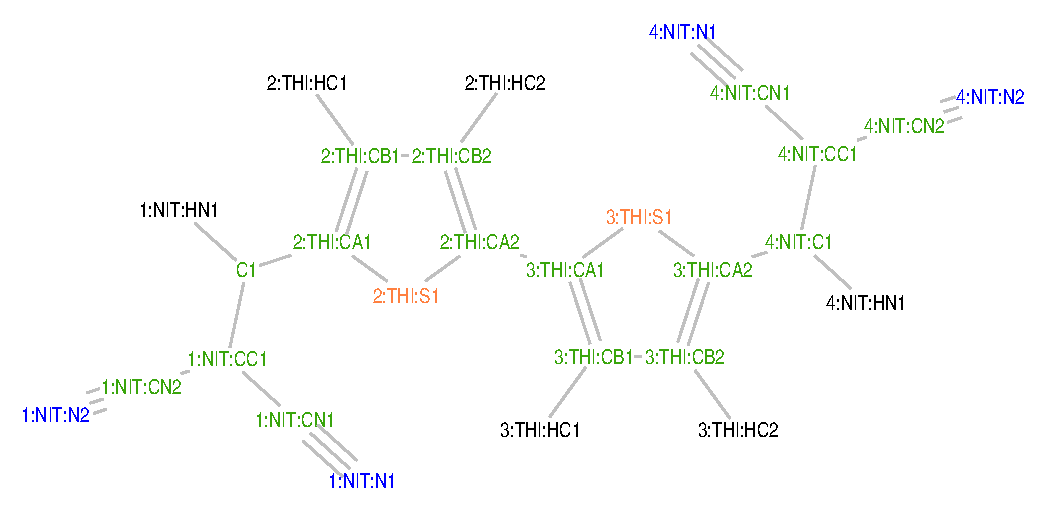
\includegraphics[width=0.9\linewidth]{./fig/chemical_structure/dcv2t_atom_types}
\caption{\small Atom types of DCV2T. The molecule consists of two building blocks (residues): thiophene (THI) and dicyanovinyl (NIT). }
\label{fig:dcv2t_at}
\end{wrapfigure}

%\clearpage
The structure of DCV2T, together with atom type definitions, is shown in fig.~\ref{fig:dcv2t_at}. DCV2T is a typical donor-acceptor-type molecule, with two electron-donating thiophene and two electron-withdrawing dicyanovinyl groups. The pdb file which contains residue types, residue numbering, atom names, atom types, and atom coordinates is shown below. In its ground state the molecule is practically planar. 

An amorphous morphology was obtained by quenching the 512 DCV2T molecules after equilibrating the system above the glass transition temperature. What we will need is a snapshot out of the trajectory and the topology file describing the system (all in GROMACS format).

%\clearpage
\lstinputlisting[
  basicstyle=\ttfamily\footnotesize,
  frame=lines,
  identifierstyle=\color{red},
  keywordstyle=\color{blue},
  showstringspaces=false,
 label=list:pdb, 
 morekeywords={HETATM,THI,NIT},
 caption={pdb file of DCV2T}]%
{./fig/chemical_structure/dcv2t.pdb}

\section{Conjugated segments}

\ctpmap partitions the system on conjugated segments and rigid fragments:
\begin{verbatim}
  ctp_map --top topology.tpr -c 15 -cg cgmap.xml --trj traj.trr
\end{verbatim}
The input are the gromacs topology and trajectory files, a mapping file, a cutoff distance for defining nearest neighbours and a file describing the charge unit types. The output includes a neighbour list, labelled by the gromacs step number, and a binary 
file and a state file with the mapped onto conjugated segments system. 

In order to check the mapping one can use the \dumptraj calculator
\begin{verbatim}
  ctp_run --exec  "dumptraj" -cg map.xml 
\end{verbatim}

This program will read in the state file created by \ctpmap together with a conjugated segment definitions and will create two output trajectory files corresponding to the coarse-grained and back-mapped topologies. The back-maping of the coase-grained topology is performed using stored rigid fragment positions and orientations. It is suggested to view all three trajectories (atomistic, coarse grained, and quantum) on top of each other to check the mapping.

\subsection{The mapping file}
To partition the system onto conjugated segments and rigid fragments a mapping \xml file is required. This file is based on the input provided for generation of \texttt{topol.tpr} and \texttt{traj.trr} files. An example of a mapping file for a single \dcvt molecule is shown in listing~\ref{list:map}. 

%\begin{table}
{\small 
\begin{tabular}{p{3cm} p{10cm}}
\xml tag & Description \\
\hline
\texttt{name} & Name of the molecule in the coarse-grained model. Useful for multicomponent systems. \\
%
\texttt{ident} & Name (identification) of the molecule in the all-atom representation. This \emph{must} match the molecule name in the atomistic representation (e.g. \gromacs topology). \\
%
\texttt{topology} & Section describing the partitioning of the molecule on rigid fragments. Atom and residue names/types \emph{must} correspond to those used in the atomistic representation (e.g. \gromacs topology)\\
& \\
\texttt{cg\_beads} & Section describing all rigid fragments of a molecule. \\
%
\texttt{cg\_bead} & Section defining one particular rigid fragment. \\
%
\texttt{cg\_bead.name} &  The name of the bead. This must be unique for each rigid fragment in a molecule, for example a polymer made of ten repeat units needs ten different name identifiers if each repeat unit is a rigid fragment. \\
%
\texttt{cg\_bead.type} &  The type of the rigid fragment. This may be the same for beads which only differ by a hydrogen atom or two to simplify the calculations, while the mapping must take these differences into account. \\
%
\texttt{cg\_bead.mapping} & The type of the mapping. Different beads may have the same mapping, since a molecule may contain multiple beads of the same type, but in the bead definition each must correspond to different atoms. \\
%
\texttt{cg\_bead.beads} &  List of all atoms belonging to the rigid fragment in the format \texttt{residue number:residue name:atom name}. Depending on the options, the first three atoms might be used to calculate vectors defining the orientation of the rigid fragment. In this case they must not lie on the same axis. Even though the first three atoms in the mapping need not correspond to the first three atoms in the \texttt{*.rtp} or \texttt{*.gro} files, the order must be consistent with the definitions in the \texttt{list\_charges} file. \\
%
\texttt{cg\_bead.symmetry} &  The symmetry of the molecule. \texttt{symmetry = 3} corresponds to a fragment with three different moments of inertia of the mass tensor. Used to automatically determine fragment orientation.\\
& \\
\texttt{qm} & This section associates rigid fragments (beads) with a particular type of a conjugated segment. \\
%
\texttt{qm.crgunitname} &  The name of the conjugated segment the fragment is associated with. \\
%
\texttt{qm.bead} & The position of the rigid fragment in the conjugated segment. \\
& \\
\texttt{maps} & Section describing maps for all types of rigid fragments. Maps are used to determine the position of a rigid fragment. \\
%
\texttt{map} &  Section defining one particular map. \\
%
\texttt{map.name} & The map name must correspond to the name used to define the fragments (\texttt{cg\_beads.mapping} tag) . \\
%
\texttt{map.weights} & The weighting of the atoms in the rigid fragment. If the mass of the nucleus in atomic mass units is used, the center of the rigid fragment will be its center of mass. The weights must be in the same order as in the corresponding rigid fragment definition (\texttt{cg\_beads.bead} tag).
\end{tabular}
}
%\end{table}

\clearpage

\definecolor{gray}{rgb}{0.4,0.4,0.4}
\definecolor{darkblue}{rgb}{0.0,0.0,0.6}
\definecolor{cyan}{rgb}{0.0,0.6,0.6}

\lstset{
  language=XML,
  frame=lines,
  basicstyle=\ttfamily\footnotesize,
  identifierstyle=\color{red},
  keywordstyle=\color{blue},
  showstringspaces=false,
  columns=fullflexible,
  commentstyle=\color{gray}\rmfamily\itshape,
  morekeywords={cg_molecule,cg_beads,cg_bead,crgunitname,bead,beads,type,topology,name,ident,maps,map,mapping,weights,position,qm,symmetry},
}

\lstinputlisting[
 label=list:map, 
 morekeywords={cg_molecule,cg_beads,name,ident,maps,map,mapping,weights,qm,symmetry},
 caption={Partitioning of DCV2T on conjugates segments and rigid fragments}]%
{./fig/mapping/cgmap.xml}

\subsection{Conjugated segments}

Conjugated segments are described in a separate \xml file. An example for \dcvt is shown in listing~\ref{list:conjugated_segments}.

\lstset{
  language=XML,
  frame=lines,
  basicstyle=\ttfamily\footnotesize,
  identifierstyle=\color{red},
  keywordstyle=\color{blue},
  showstringspaces=false,
  columns=fullflexible,
  commentstyle=\color{gray}\rmfamily\itshape,
  morekeywords={crgunit_type,ChargeUnitType,posname,orbname,basisset,transorb,reorg,nameneutr,namecrg,energy,beadconj,molname,name,monomer_atom_map,monomer_atom_weights},
}

\lstinputlisting[
 label=list:conjugated_segments, 
 caption={\small \xml file describing conjugated segments.
}]%
{./fig/moo/charges.xml}

\noindent
\suggestion{%
crgunit\_type -> ConjugatedSegmentTypes \\ 
ChargeUnitType -> ConjugatedSegmentType \\ 
posname -> CoordinatesFile \\
orbname -> OrbitalsFile \\
transorb -> TransportOrbital \\
reorg -> ReorganizationEnergy (do we need this here?) \\
nameneutr -> ChargesNeutralFile \\
namecrg -> ChargesChargedFile (do we need this here?) 
}

{\small 
\begin{tabular}{p{3cm} p{10cm}}
\xml tag & Description \\
\hline
 \texttt{posname} & Location of \xyz. \\
 \texttt{orbname} & Location of \orb. \\
 \texttt{basisset} & This should be set to INDO, unless the fort.7 has been created using another basis set. In that case it must be set to an \xml file setting the characteristics of the basis set. \\
 \texttt{transorb} & Number of HOMO (LUMO) orbital. Corresponds to the number of $\alpha$ electrons in the \gaussian log-file {get\_orbitals.log} minus one (since counting in C++ starts at zero) for the HOMO and the number of $\alpha$ electrons for the LUMO. \\
 \texttt{reorg} & Reorganization energy of the cation or anion in eV. \\
 \texttt{name} & Name of the mapping of the molecule. Must correspond to CG mapping.\\
 \texttt{energy} & Site energy of the conjugated segment. \\
 \texttt{monomer\_atom\_map} &
 List of atom indices as they were specified in the \gaussian input used to create the \orb file. 
 Note: The first three values are important, since they must correspond to the first three atoms defined in the coarse-grained mapping, which are used to calculate two vectors indicating the orientation of the molecule. The third required vector is the eigenvector of the smallest eigenvalue of the gyration tensor, i.e. perpendicular to the planar core.
 Note: The number of molecules here may differ from that in the coarse-grained mapping, since for example only the core is important for transport and not the side chains, but it has to be the same number of atoms as in the \gaussian input file otherwise overlap integral values will be terribly wrong. 
\end{tabular}




\chapter{Calculators}
\label{sec:prog_interf}
\subsection{Calculators}
\label{sec:calculators}

Calculator is a piece of code which computes specific system properties, such as site energies, transfer integrals, etc. \ctprun is a wrapper program which executes all calculators. The generic syntax is 
\begin{verbatim}
  ctp_run --exec "calc1, calc2, ..." --opt options.xml
\end{verbatim}
%
File \texttt{options.xml} lists all options needed to run a specific calculator. The format of this file is explained in listing~\ref{list:calc}. A complete list of calculators is given in the \refcalc reference section.
%
\lstinputlisting[label=list:calc, 
 caption={\small A part of the \texttt{options.xml} file with options for the \texttt{calculator\_name\{1,2\}} \refcalc.
}]{./programs/calculators.xml}


\chapter{Reference}
\label{sec:reference}
\section{Programs}
\label{ref:programs}
\label{sec:programs}
Programs execute specific tasks (calculators). 

%\input{reference/programs/all}

\section{Calculators}
\label{ref:calculators}
\label{sec:calculators}

Calculator is a piece of code which computes specific system properties, such as site energies, transfer integrals, etc. \xtprun, \kmcrun are wrapper programs which executes such calculators. The generic syntax is 
\vskip 0.2cm
{\noindent \small \xtprun \exe \texttt{"calc1, calc2, ..."} \opt \xmloptions }
\vskip 0.2cm
%
File \xmloptions lists all options needed to run a specific calculator. The format of this file is explained in listing~\ref{list:calc}. A complete list of calculators is given in the \refcalc reference section.
%
\lstinputlisting[label=list:calc, 
 caption={\small A part of the \xmloptions file with options for the \texttt{calculator\_name\{1,2\}} \refcalc.
}]{./reference/calculators.xml}

A list of all calculators and their short descriptions can be obtain using 
\vskip 0.1cm
{\noindent \small \xtprun \texttt{-{}-list} }
\vskip 0.1cm

A detailed description of all options of a specific calculator(s) is available via
\vskip 0.1cm
{\noindent \small \xtprun \texttt{-{}-desc calc1,calc2,...} }

%\subsection{Calculators}
\label{sec:calculators}

Calculator is a piece of code which computes specific system properties, such as site energies, transfer integrals, etc. \ctprun is a wrapper program which executes all calculators. The generic syntax is 
\begin{verbatim}
  ctp_run --exec "calc1, calc2, ..." --opt options.xml
\end{verbatim}
%
File \texttt{options.xml} lists all options needed to run a specific calculator. The format of this file is explained in listing~\ref{list:calc}. A complete list of calculators is given in the \refcalc reference section.
%
\lstinputlisting[label=list:calc, 
 caption={\small A part of the \texttt{options.xml} file with options for the \texttt{calculator\_name\{1,2\}} \refcalc.
}]{./programs/calculators.xml}

\vfill

\section{Common options}
\label{ref:options}
%\setdefaultleftmargin{0.8em}{0.8em}{0.8em}{0.8em}{0.8em}{0.8em}
\rowcolors{1}{invisiblegray}{white}
{\small 
%\input{reference/xml/options.xml}
}
\vfill


\appendix
\newcommand{\indM}{l} 
\newcommand{\indN}{m}
\newcommand{\lb}[1]{\langle #1 |}
\newcommand{\rb}[1]{| #1 \rangle}
\newcommand{\rbt}[1]{ #1 \rangle}

%\appendixpage
%\addappheadtotoc
\chapter{Bimolecular electron transfer rate}
\label{sec:rate_bimolecular}

\begin{figure*}[ht]
%    \includegraphics[width=1.0\textwidth]{fig/jortner_rate/marcus_parabolas_new}
   \caption{
(a) Potential energy surfaces of the charge transfer complex in a dimer representation. ET is from molecule $i$ to molecule $j$. In the initial state, $\rb{I_{00}}$, both molecules are in their vibrational ground states. In the final state, $\rb{F_{l'm'}}$, the neutral molecule $i$ is in vibrational state $l'$, while the charged molecule $j$ is in vibrational state $m'$. Initial and final states are coupled to a classical harmonic outer-sphere normal mode with mass weighted average coordinate $q$ and reorganization energy $\lambda_{ij}^\text{out}$. For small couplings $V_{I_{00}F_{l'm'}}$ the ET reaction takes place on the diabatic states (solid curves). 
%
(b) PES of molecule $i$ as a function of the averaged normal mode $q_i$. $l$ and $l'$ enumerate vibrational modes of the initial charged and the final neutral states. (c) Same as (b) for initially neutral molecule $j$. 
%
$\Delta U_i$ ($\Delta U_j$) is the internal energy difference while $\lambda_i^{cn}$ ($\lambda_j^{nc}$) is the  intramolecular reorganization energy for discharging molecule $i$ (charging molecule $j$). }
   \label{fig:marcus_parabolas}
\end{figure*}

In the case of a bimolecular electron transfer (ET) reaction the electron moves between two independent molecules. Therefore, one needs separate sets of coordinates for the donor and acceptor. Strictly speaking, the classical Marcus rate assumes a common set of vibrational coordinates and, as such, can not be used for bimolecular ET. Yet if the independent vibrational modes are harmonic, are treated classically, and the charging and discharging reorganization energies of the molecule are identical, one still obtains the Marcus-type ET rate with the intramolecular reorganization energy which is the sum of the reorganization energies of the donor and the acceptor~\cite{may_charge_2003}. Similarly, the classical treatment of the outer-sphere mode, which is due to rearrangement of the surrounding, allows to add its reorganization energy  to the intramolecular one.

However, the main issue with the classical Marcus rate is that the high-frequency intramolecular vibrational modes are energetically comparable to the C-C bond stretching mode. At room temperature $\hbar \omega_\text{CC} \sim 0.2\, \unit{eV} \gg k_\text{B}T \sim 0.025\, \unit{eV}$  and therefore these modes should be treated quantum mechanically. In fact, for a common set of intramolecular high-frequency  (quantum-mechanical) and an outer sphere low-frequency (classical) vibrational coordinates, a mixed quantum-classical multi-channel generalization of the Marcus formula is readily available~\cite{may_charge_2003}. Such generalization,  to the best of our knowledge, has not been made for the bimolecular ET rate, which requires independent sets of coordinates for donor and acceptor. The purpose of this section is to derive a quantum-classical expression for the ET rate with two independent, high-frequency vibrational modes and a common low-frequency outer sphere mode. 

Following Ref.~\cite{bredas_charge-transfer_2004} we assume that all intramolecular modes of a donor $i$ can be averaged into a mode with mass weighted coordinate ${q_i}$ and energy $\hbar\omega^{n}_i$ ($\hbar\omega^{c}_i$) for the molecule in a neutral (charged) state. Similar assumptions are made for the acceptor $j$. In addition, we allow for an averaged classical outer-sphere mode with mass weighted coordinate ${q}$ and energy $\hbar\omega^\text{out}_{ij}\ll k_\text{B}T$. This mode is common to both molecules and plays the role of the ET reaction coordinate~\cite{note_outer}.

In amorphous organic semiconductors the electronic coupling is usually small compared to both the energy of the classical vibrational mode and intermolecular reorganization energies. In this case the initial, $ \rb{I_{\indM\indN}}$, and final, $\rb{F_{\indM'\indN'}}$, states of the ET reaction are diabatic (non-interacting) dimer states which depend on the vibrational states (with quantum numbers $\indM, \indN, \indM, '\indN'$) of both molecules. The potential energy surfaces (PES) corresponding to these states are shown in \fig{marcus_parabolas}a. The PES for intramolecular degrees of freedom for molecules $i$ and $j$ are shown in \fig{marcus_parabolas}b and c, respectively.

For the contributions of the outer-sphere mode to initial and final states we introduce Hamiltonian functions
\begin{equation}
 H_{I,F}(q)=\frac{1}{2}\left[ \omega^\text{out} \left( q-q_{I,F} \right) \right]^2 \, ,
\end{equation}
where the equilibrium position in the initial (final) state $q_I$ ($q_F$) corresponds to the arrangement of all nuclear coordinates of molecules surrounding the ET complex when molecule $i$ ($j$) is charged.  The outer sphere reorganization energy, defined as $\lambda^\text{out}_{ij}=\frac{1}{2}\left[ \omega^\text{out}|q_I-q_F| \right]^2$,  is shown in~\fig{marcus_parabolas}a. It can be computed from the initial and final electric displacement fields of the charge-transfer complex. 

The complete Hamiltonian of the ET complex can now be written as
\begin{equation}
\begin{split}
 H_{ij}=&\hphantom{+}\sum_{\indM,\indN=0}^\infty \left( H_I(q) + E^{ij}_{\indM\indN} \right) \rb{I_{\indM\indN}} \lb{I_{\indM\indN}} %\\
        +\sum_{\indM',\indN'=0}^\infty \left( H_F(q) + E^{ji}_{\indN'\indM'} \right) \rb{F_{\indM'\indN'}} \lb{F_{\indM'\indN'}} %\\
        +\sum_{\indM,\indN,\indM',\indN'}V_{I_{\indM\indN}F_{\indM'\indN'}} \rb{I_{\indM\indN}} \lb{F_{\indM'\indN'}} +\text{h.c} \,, \\
 E^{ij}_{\indM\indN}=& \hphantom{+} U_i^{cC} + U_j^{nN} + E_i^\text{el} + E_i^\text{ext}
+ \hbar\left[\omega_i^c\left(\indM+\frac{1}{2}\right) + \omega_j^n\left(\indN+\frac{1}{2}\right) \right] \, , 
       \\
 E^{ji}_{\indN'\indM'}=&\hphantom{+} U_j^{cC} + U_i^{nN} + E_j^\text{el} + E_j^\text{ext} 
+ \hbar\left[\omega_j^c\left(\indN'+\frac{1}{2}\right) +\omega_i^n\left(\indM'+\frac{1}{2}\right)\right] \, .
\end{split}
\label{equ:hami}
\end{equation}
Here, a manifold of initial states, $\rb{I_{\indM \indN}} $, with quantum numbers $\indM$ ($\indN$) for intramolecular vibrations in molecule $i$ ($j$) and energy $E^{ij}_{\indM \indN}$, is coupled to a classical phonon bath $H_I(q)$. Transitions to the manifold of final states  $\rb{F_{\indM' \indN'}} $ where the charge has hopped from $i$ to $j$ are possible due to a coupling $V_{I_{\indM\indN}F_{\indM'\indN'}} $.
The initial, $E^{ij}_{\indM\indN}$,  and final, $E^{ji}_{\indN'\indM'}$, energies contain internal energies $U_i^{nN}$ and $U_i^{cC}$ ($U_j^{nN}$ and $U_j^{cC}$) of molecule $i$ (molecule $j$) in the neutral and charged ground states, the contributions of the external electric field, $E_i^\text{ext}$ and $E_j^\text{ext}$, and electrostatic interactions, $E_i^\text{el}$ and $E_j^\text{el}$, and respective oscillator energies.  

Within the Born-Oppenheimer approximation, a separation in terms of electronic and nuclear degrees of freedom gives
\begin{equation}
\begin{split}
 \rb{I_{\indM\indN}}&=\rb{\phi_i^c}\rb{\chi_{i\indM}^c}\rb{\phi_j^n}\rb{\chi^n_{j\indN}}\, ,\\
 \rb{F_{\indM'\indN'}}&=\rb{\phi^n_i}\rb{\chi^n_{i\indM'}}\rb{\phi_j^c}\rb{\chi_{j\indN'}^c}\, ,
\end{split}
\end{equation}
where $\phi_i^n$ ($\phi_i^c$) corresponds to the electronic part of the wave function, while $\chi_{i\indM}^n$  ($\chi_{i\indM}^c$) represents an $\indM$-th phonon mode of the neutral (charged) molecule $i$.

The coupling element $V_{I_{\indM\indN}F_{\indM'\indN'}}$ in~\equ{hami} can then be factorized in an electronic and nuclear parts 
\begin{equation}
V_{I_{\indM\indN}F_{\indM'\indN'}}=J_{ij} \lb{\chi_{i\indM}^c}\rbt{\chi_{i\indM'}^n} \lb{\chi_{j\indN}^n}\rbt{\chi_{j\indN'}^c}\,.
\end{equation}
Franck-Condon overlap integrals $\lb{\chi_{i\indM}^c}\rbt{\chi_{i\indM'}^n}$ ($\lb{\chi_{j\indN}^n}\rbt{\chi_{j\indN'}^c} $) describe couplings of vibrational modes $\indM,\indM'$ ($\indN,\indN'$) of the charged and neutral configurations of molecule $i$  ($j$). Exemplary modes are shown in~\fig{marcus_parabolas}b,c.

Since $k_\text{B}T\ll \hbar\omega_i^{c},\hbar\omega_j^{n}$ one can restrict the initial state to the vibrational ground-states $\indM=\indN=0$ while allowing tunneling to all vibrationally excited states $\indM'$ for molecule $i$ and $\indN'$ for molecule $j$. In other words, a single initial state $\rb{I_{00}}$ couples to a manifold of final states $\rb{F_{\indM',\indN'}}$. 
%
This assumes that ET is sufficiently slow compared to the relaxation of the intramolecular degrees of freedom, so that there is enough time for a complex to relax to its vibrational ground state between two consecutive ETs. 

The energy difference driving the reaction to channel ${\indM'\indN'}$  therefore is
\begin{equation*}
 \Delta E^{ij}_{\indM'\indN'}= E^{ij}_{00}-E^{ji}_{\indN'\indM'}=\Delta E_{ij} - \hbar (\omega_i^n\indM'+\omega_j^c\indN')\,,
\end{equation*}
where $\Delta E_{ij}=\Delta E_{ij}^\text{ext}+\Delta E_{ij}^\text{el}+\Delta E^\text{int}_{ij}$.

Assuming that $|V_{I_{00}F_{\indM'\indN'}}|\ll\lambda_{ij}^\text{out},\hbar\omega^\text{out}$ and using Fermi's golden rule with $V_{I_{00}F_{\indM'\indN'}}$ as a perturbation to the initial diabatic state, we obtain a multi-channel rate equation
\begin{equation}
%\begin{split}
\omega_{ij}=\sum_{\indM',\indN'=0}^\infty \frac{2\pi}{\hbar}|V_{I_{00}F_{\indM'\indN'}}|^2 
% \times  
\int dq f_I(q) \delta(\Delta E^{ij}_{\indM'\indN'} + H_I(q) -H_F(q))\, .
%\end{split}
\end{equation}
where the thermal averaging over the classical outer-sphere mode is performed by introducing a  canonical distribution function  $f_I(q)=Z^{-1}\exp(-H_I(q)/k_\text{B}T)$, with $Z=\int{dq \exp(-H_I(q)/k_\text{B}T)}$.

Energy conservation pins the transition to the crossing point of the diabatic PES (see~\fig{marcus_parabolas}a) resulting in 
\begin{eqnarray}
 \omega_{ij}= \frac{2\pi}{\hbar}  \frac{|J_{ij}|^2}{\sqrt{4\pi \lambda_{ij}^\text{out} k_\text{B}T}} 
 \sum_{\indM',\indN'=0}^\infty
 |\lb{\chi_{i0}^c}\rbt{\chi_{i\indM'}^n}|^2 |\lb{\chi_{j0}^n}\rbt{\chi_{j\indN'}^c}|^2 
%\nonumber \\&& 
\exp
\left\{ -\frac{ \left[ \Delta E_{ij}-\hbar(\indM'\omega_i^n+\indN'\omega_j^c) -\lambda_{ij}^\text{out} \right]^2}{4\lambda_{ij}^\text{out} k_\text{B}T}
\right\} .
\label{equ:jjortner}
\end{eqnarray}
\Equ{jjortner} is the quantum-classical expression for the bimolecular ET rate with two independent, high-frequency vibrational modes and one classical common outer-sphere mode. It is the main result of this section. 

If the curvatures of intramolecular PES of charged and neutral states of a molecule are different, that is $\omega_i^c\neq\omega_i^n$, the corresponding reorganization energies, $\lambda_i^{cn}=\frac{1}{2}[\omega_i^n(q_i^n-q_i^c)]^2$ and $\lambda_i^{nc}=\frac{1}{2}[\omega_i^c(q_i^n-q_i^c)]^2$, will also differ. In this case the Franck-Condon (FC) factors for discharging of molecule $i$ read \cite{chang_new_2005}
\begin{equation}
%\begin{split}
%&
|\lb{\chi_{i0}^c}\rbt{\chi_{i\indM'}^n}|^2 = 
\frac{2}{2^{l'}l'!} \frac{\sqrt{\omega_i^c\omega_i^n}}{(\omega_i^c+\omega_i^n)} \exp\left( -|s_i| \right)
%\nonumber \\
%& \times
 \left[ \sum_{\substack{k=0\\k\,\text{even}}}^{\indM'} {\indM' \choose k} 
\left( \frac{2 \omega_i^c }{\omega_i^c+\omega_i^n}\right)^{k/2} \frac{k!}{(k/2)!}
H_{\indM'-k} \left( \frac{s_{i}}{\sqrt{2S^{cn}_i}}\right) 
\right]^2
\, ,
%\end{split}
\end{equation}
where $H_n(x)$ is a Hermite polynomial, $s_i=\frac{2\sqrt{\lambda_i^{nc}\lambda_i^{cn}}}{\hbar(\omega_i^c+\omega_i^n)}$, and $S^{cn}_i=\lambda_i^{cn}/\hbar\omega_i^c$. The FC factors for charging of molecule $j$ can be obtained by substituting $(s_i,S^{cn}_i,\omega_i^c)$ with $(-s_j,S^{nc}_j, \omega_j^n)$. In order to evaluate the FC factors, the internal reorganization energy $\lambda_i^{cn}$ can be computed from the intramolecular PES, as shown in~\fig{marcus_parabolas}b,c. 

To conclude the section, we compare the bimolecular quantum-classical rate, \equ{jjortner}, the classical bimolecular Marcus rate, eq.~(1) of the main text, and the quantum-classical Jortner rate with a common set of vibrational coordinates~\cite{may_charge_2003}
\begin{eqnarray}
 \omega_{ij} = \frac{2\pi}{\hbar}  \frac{|J_{ij}|^2}{\sqrt{4\pi \lambda_{ij}^\text{out} k_\text{B}T}} 
 \sum_{N=0}^\infty \frac{1}{N!} \left( \frac{\lambda_{ij}^\text{int}}{\hbar\omega^\text{int}} \right)^{N} 
  \exp \left( - \frac{\lambda_{ij}^\text{int}}{\hbar\omega^\text{int}}\right) 
%\nonumber\\&& 
\exp
\left\{ -\frac{ \left[ \Delta E_{ij}-\hbar N\omega^\text{int} -\lambda_{ij}^\text{out} \right]^2}{4\lambda_{ij}^\text{out} k_\text{B}T}
\right\} .
\label{equ:jortner}
\end{eqnarray}

If $\omega_i^c=\omega_i^n=\omega_i$ ($\lambda_i^{nc}=\lambda_i^{cn}=\lambda_i$), the Franck-Condon factor simplifies to
\begin{equation}
|\lb{\chi_{i0}}\rbt{\chi_{i\indM'}}|^2 = \frac{1}{\indM'!} \left( \frac{\lambda_i}{\hbar\omega_i} \right)^{\indM'} \exp \left( - \frac{\lambda_i}{\hbar\omega_i}\right)\,.
\end{equation}
If this simplification is applicable for both donor and acceptor molecules,  \equ{jjortner} becomes identical to the quantum-classical rate~\equ{jortner} with $\lambda_{ij}^\text{int}=\lambda_i+\lambda_j$.

\begin{figure*}[ht]
%   \includegraphics[width=\linewidth]{fig/jortner_rate/compare_rates}
   \caption{ (a) Scaled hopping rates, $\bar{\omega}_{ij} = \omega_{ij}  J_{ij}^{-2} (2\pi)^{-1} \hbar\sqrt{4\pi k_\text{B}T}$, calculated using the classical Marcus, Jortner quantum mechanical~\equ{jortner} and bimolecular multichannel~\equ{jjortner} rate expressions. 
%
Outer sphere reorganization energy $\lambda_{ij}^\text{out}=0.05\, \unit{eV}$,  $\lambda^{cn}_i=\lambda_j^{cn}=0.14\, \unit{eV}$, and $\lambda^{nc}_i=\lambda^{nc}_j=0.09\, \unit{eV}$ (all added in the classical Marcus rate while the latter two are added for the Jortner rate). 
%
Intramolecular vibrations have averaged frequency $\hbar\omega_i^\text{int}=\hbar\omega_j^\text{int}=0.2\, \unit{eV}$ for the Jortner rate while $\hbar\omega_i^n=0.2\, \unit{eV}$ and $\hbar\omega_j^c=\hbar\omega_i^n \sqrt{\lambda_j^{nc}}/\sqrt{\lambda_j^{cn}}$ for the bimolecular rate. 
%
(b) The same but for $\lambda_{ij}^\text{out}=0.1\, \unit{eV}$. 
%
(c) Histogram of rates at a field of $10^8\, \unit{Vm^{-1}}$ for the Marcus and Jortner rates with distance dependent $\lambda_{ij}^\text{out}<0.08\, \unit{eV}$ for the neighborlist pairs and constant $\lambda^\text{int}=0.23\, \unit{eV}$. A small difference can be seen in the tail of small rates.}
   \label{fig:mj_comparison}
\end{figure*}

% discussion of the equation
To compare the quantum-mechanical and classical rates, intramolecular hole reorganization energies of \Alq, $\lambda^{cn}_i=0.14\,\unit{eV}$ and $\lambda^{nc}_i=0.09\,\unit{eV}$ were used. We also assumed that $\omega_i^n=0.2\,\unit{eV}$ and $\omega_i^c=\omega_i^n\sqrt{\lambda^{nc}_i / \lambda^{cn}_i}$. Due to the uncertainty in determining $\lambda_{ij}^\text{out}$, two cases are considered, $\lambda_{ij}^\text{out}=0.05\,\unit{eV}$ (\fig{mj_comparison}a) and $\lambda_{ij}^\text{out}=0.10\,\unit{eV}$ (\fig{mj_comparison}b). Note that the estimate made in the main text predicts $\lambda_{ij}^\text{out} < 0.08\,\text{eV}$. In both cases we used fixed, molecular-separation independent, $\lambda_{ij}^\text{out}$. 

\Fig{mj_comparison} shows that the main difference between the quantum-classical and classical rates is the tail of smaller rates for large negative $\Delta E$ (endothermal hopping) and higher rates for large positive $\Delta E$ (exothermal hopping).  \Fig{mj_comparison}c also shows the corresponding distributions of rates for all pairs from the neighbor list for 512 molecules of  amorphous \Alq. Here we used the distance-dependent $\lambda_{ij}^\text{out}$ from the neighbor list as computed from dielectric displacement fields with the Pekar factor of $c_p=0.01$. One can see that the distributions are practically on top of each other (except for very small rates) and hence will lead to similar charge dynamics. 

In general, our observation is that for a situation with (i) intramolecular reorganization energy similar to the outer sphere one ($\lambda_{ij}^\text{int} \sim \lambda_{ij}^\text{out}$), (ii) driving force $\Delta E_{ij}$ small compared to the intramolecular reorganization energy, and (iii) $\lambda \sim \hbar \omega$, the classical (eq.~(1) of the main text) and semi-classical  (\equ{jortner} and \equ{jjortner}) expressions lead to quantitatively similar rates.
However, for systems with large $\Delta E_{ij}$, such as donor-acceptor mixtures, \equ{jjortner} or \equ{jortner} should be used. In this case a rather accurate estimate of the outer sphere reorganization energy is required~\cite{mcmahon_evaluation_2010}.



\bibliographystyle{achemso}
\bibliography{literature_short}

\end{document} 
